\documentclass[12pt, psamsfonts]{amsart}

%-------Packages---------
\usepackage{amssymb,amsfonts}
\usepackage{fullpage}
\usepackage{todonotes}
\usepackage{physics}
\usepackage[all,arc]{xy}
\usepackage{enumerate}
\usepackage{mathrsfs}
\usepackage{theoremref}
\usepackage{graphicx}
\usepackage[bookmarks]{hyperref}

%--------Theorem Environments--------
%theoremstyle{plain} --- default
\newtheorem{thm}{Theorem}[section]
\newtheorem{cor}[thm]{Corollary}
\newtheorem{prop}[thm]{Proposition}
\newtheorem{lem}[thm]{Lemma}
\newtheorem{conj}[thm]{Conjecture}
\newtheorem{quest}[thm]{Question}

\theoremstyle{definition}
\newtheorem{defn}[thm]{Definition}
\newtheorem{defns}[thm]{Definitions}
\newtheorem{con}[thm]{Construction}
\newtheorem{exmp}[thm]{Example}
\newtheorem{exmps}[thm]{Examples}
\newtheorem{notn}[thm]{Notation}
\newtheorem{notns}[thm]{Notations}
\newtheorem{addm}[thm]{Addendum}
\newtheorem*{exer}{Exercise}

\theoremstyle{remark}
\newtheorem{rem}[thm]{Remark}
\newtheorem{rems}[thm]{Remarks}
\newtheorem{warn}[thm]{Warning}
\newtheorem{sch}[thm]{Scholium}

\DeclareMathOperator{\Hom}{Hom}
\DeclareMathOperator{\Id}{Id}

\makeatletter
\let\c@equation\c@thm
\makeatother
\numberwithin{equation}{section}

\bibliographystyle{plain}

\begin{document}

\title{Math 611 Homework (Due 9/25)}
\author{Hidenori Shinohara}
\maketitle

\begin{exer}{(Problem 4, Chapter 1.3)}
  Construct a simply-connected covering space of the space $X \subset \mathbb{R}^3$ that is the union of a sphere and a diameter.
  Do the same when $X$ is the union of a sphere and a circle intersecting it in two points.
\end{exer}

\begin{proof}
  \begin{figure}
    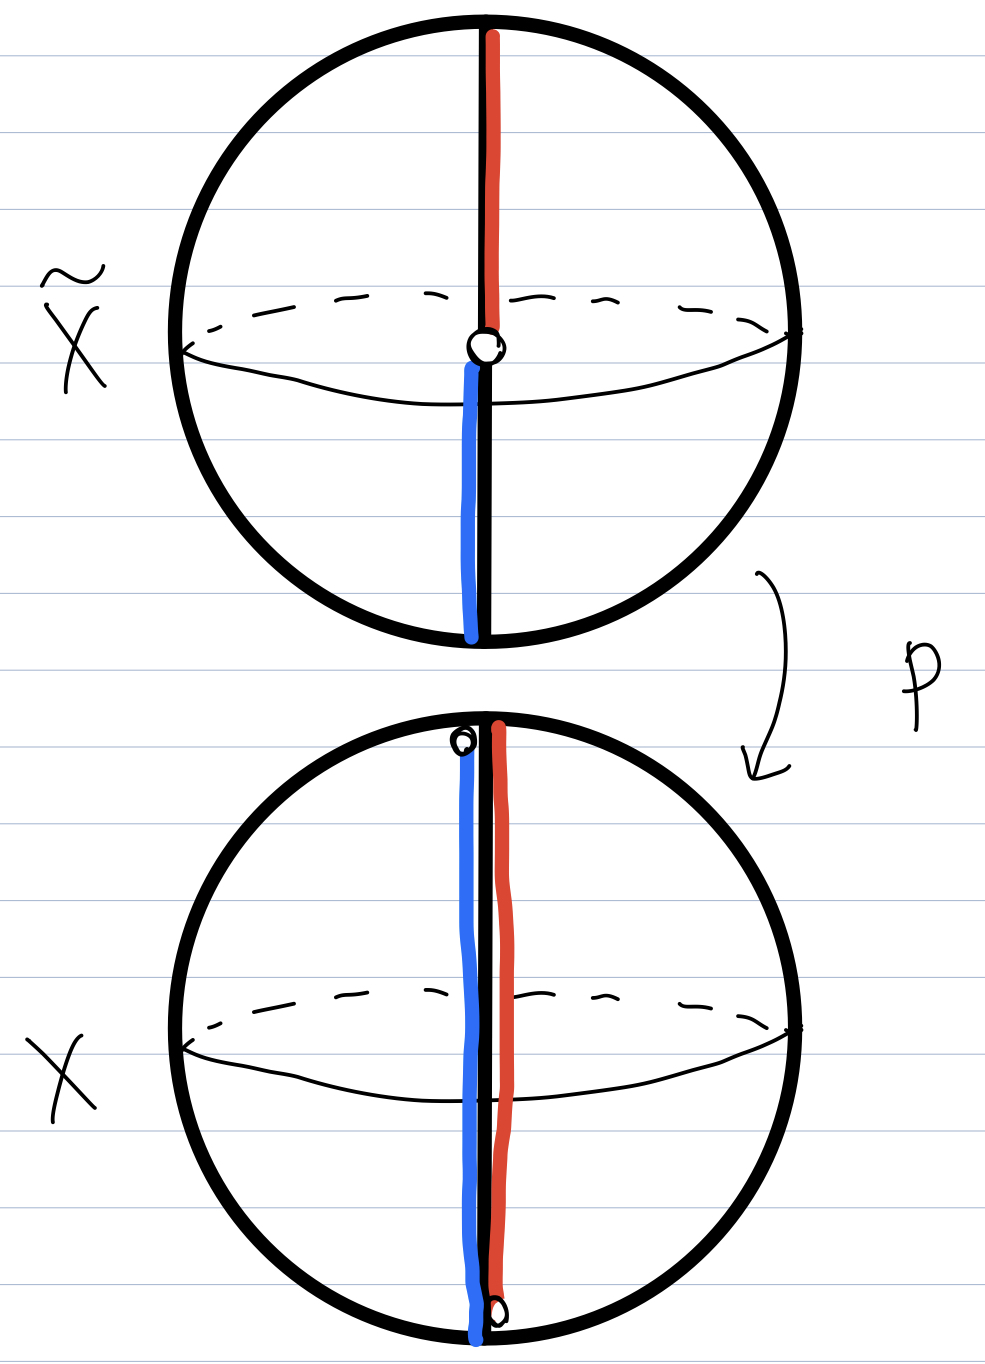
\includegraphics[width=.5\linewidth]{problem4-1.jpeg}
    \caption{Problem 4 (Part 1)}
    \label{fig:prob4_1}
  \end{figure}
  We claim that the space described in Figure \ref{fig:prob4_1} is a covering space of $X$.
  \begin{itemize}
    \item
      The shape is an infinitely long chain of spheres and lines.
      The chain goes infinitely both ways (up and down).
      Let $g$ be a loop in this space.
      Then $g$ is contained in finitely many spheres and line segments.
      Since spheres and line segments are simply connected, a finitely long chain of them is simply connected by Van Kampen.
      Therefore, $g$ is homotopic to the constant loop, thus this space is simply connected.
    \item
      We will map each sphere to the sphere of $X$.
      Each line will be mapped to the diameter up side down.
      Figure \ref{fig:prob4_1} shows how each part gets mapped.
    \item
      We claim that such a mapping is a covering map and thus this infinite chain is indeed a covering space.
      Let $x \in X$.
      \begin{itemize}
        \item
          If $x$ is on the diameter and disjoint from the sphere, a neighborhood that is disjoint from the sphere is evenly covered.
        \item
          If $x$ is on the sphere and disjoint from the diameter, a neighborhood that is disjoint from the diameter is evenly covered.
        \item
          If $x$ is the north pole, a neighborhood that does not contain the south pole is evenly covered.
        \item
          If $x$ is the south pole, a neighborhood that does not contain the north pole is evenly covered.
      \end{itemize}
  \end{itemize}
  Therefore, the space described in Figure \ref{fig:prob4_1} is a covering space of $X$.
  \begin{figure}
    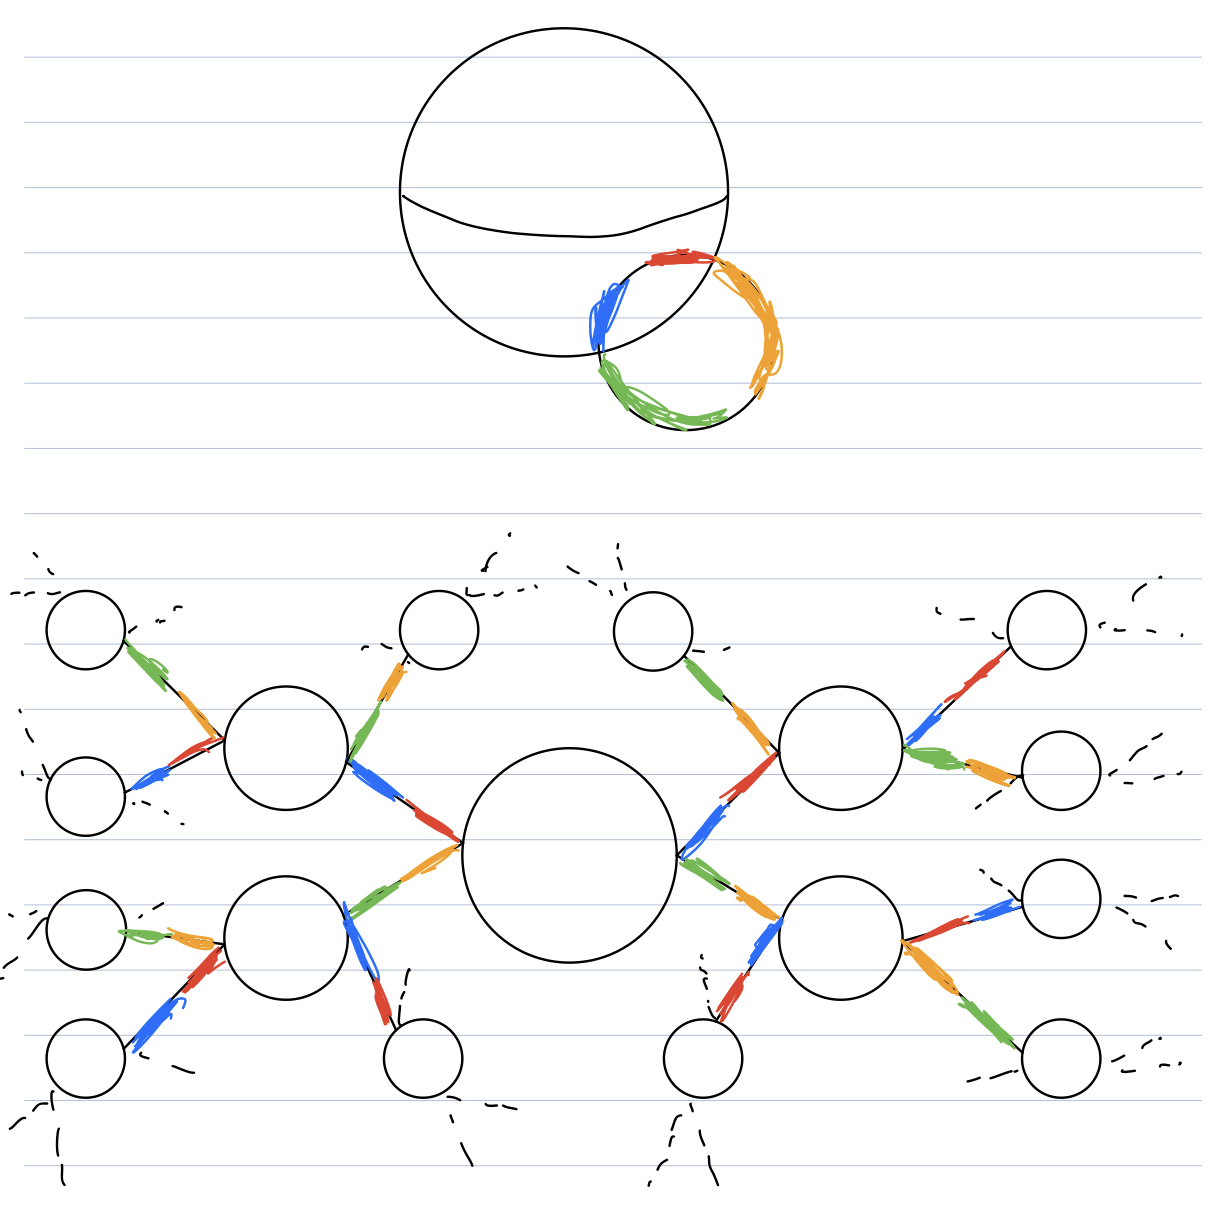
\includegraphics[width=.5\linewidth]{problem4-2.jpeg}
    \caption{Problem 4 (Part 2)}
    \label{fig:prob4_2}
  \end{figure}

  Figure \ref{fig:prob4_2} has an example of a simply-connected covering space of $X$.
  This space can be constructed by first having a sphere in the middle.
  4 edges should be attached at two points of the sphere.
  And each edge should be connected to a different sphere.
  We continue attaching them such that each sphere has exactly two points each of which has two edges.
  The edges should be mapped to the circle as described in \ref{fig:prob4_2} by 4 different colors.
  It is clear that each point has an evenly covered neighborhood.
\end{proof}

\begin{exer}{(Problem 5, Chapter 1.3)}
  Let $X$ be the subspace of $\mathbb{R}^2$ consisting of the four sides of the square $[0, 1] \times [0, 1]$ together with the segments of the vertical lines $x = 1/2, 1/3, 1/4, \cdots$ inside the square.
  Show that for every covering space $X \rightarrow X$ there is some neighborhood of the left edge of $X$ that lifts homeomorphically to $\tilde{X}$.
  Deduce that $X$ has no simply-connected covering space.
\end{exer}

\begin{proof}
  For each $y \in [0, 1]$, the point $(0, y)$ has a neighborhood $U_y$ that is evenly covered.
  Then there exists an open rectangle $R_y \subset \mathbb{R}^2$ such that $y \in R_y \cap Y \subset U_y$.
  Since any open subset of an evenly covered set is evenly covered, such $R_y \cap Y$ is evenly covered.
  Let $V_y$ denote $R_y \cap Y$ for each $y$.
  $\{ V_y  \mid y \in [0, 1] \}$ is an open cover of the segment $\{ 0 \} \times [0, 1]$.
  Since the segment is compact, there exists a finite subcover, $V_{y_1}, \cdots, V_{y_k}$.

  For simplicity, we will just call the $V_1, \cdots, V_k$ and assume that $V_1$ contains the point $(0, 0)$ and $V_k$ contains the point $(0, 1)$ and $V_i$ and $V_{i + 1}$ have a nonempty intersection.
  See Figure \ref{fig:problem5}.
  \begin{figure}
    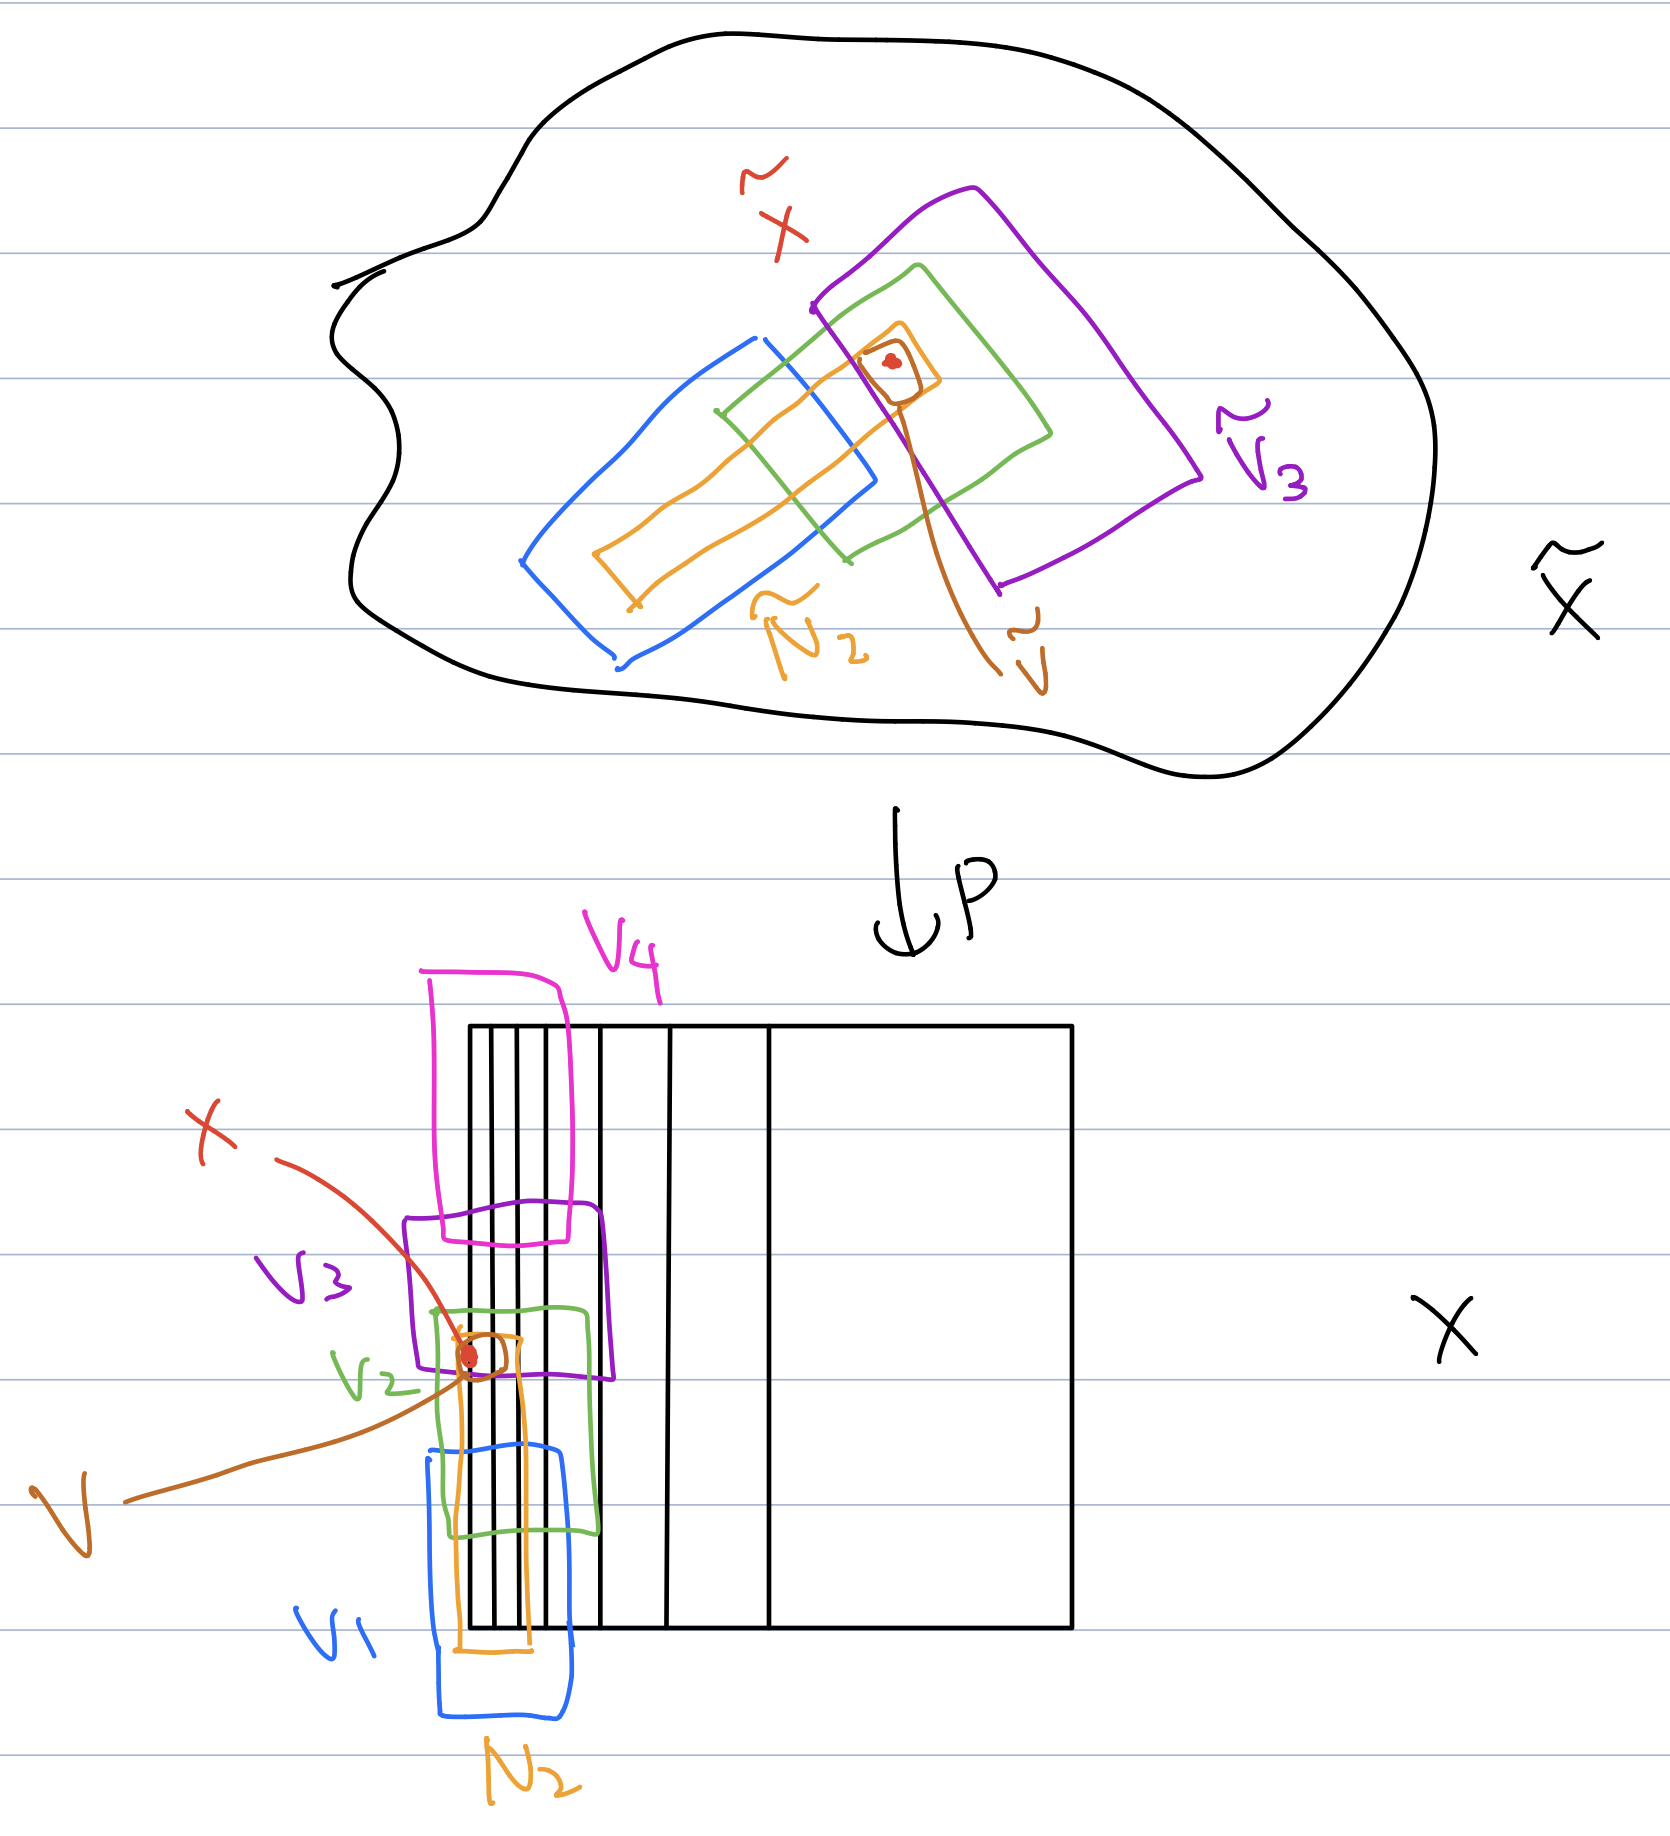
\includegraphics[width=.5\linewidth]{problem5.jpeg}
    \caption{Problem 5}
    \label{fig:problem5}
  \end{figure}

  We will construct a neighborhood of the left edge that lifts homeomorphically to $\tilde{X}$ in $k$ steps.
  $N_1 = V_1$ is a neighborhood that lifts homeomorphically.
  Let $\tilde{N}_1$ denote some open set in $\tilde{X}$ such that $p$ maps $\tilde{N_1}$ to $N_1$ homeomorphically.

  Suppose that we have constructed open sets $N_i \subset X, \tilde{N_i} \subset \tilde{X}$ for some $1 \leq i < k$.
  Let $x$ be a point in the left edge such that $x \in N_i \cap V_{i + 1}$.
  Then there exists $\tilde{x} \in \tilde{X}$ such that $\tilde{x} \in \tilde{N_i} \cap \tilde{V}_{i + 1}$ where $\tilde{V}_{i + 1}$ is some open set in $\tilde{X}$ such that $p$ maps $\tilde{V}_{i + 1}$ to $V_{i + 1}$ homeomorphically.
  Since $\tilde{N}_i$ and $\tilde{V}_{i + 1}$ are both open sets, the intersection $\tilde{V} = \tilde{N}_i \cap \tilde{V}_{i + 1}$ is a neighborhood of $\tilde{x}$.
  Then $V = p(\tilde{V})$ is a neighborhood of $x$ that is contained in $N_i$ and $V_{i + 1}$, and $p$ maps $\tilde{V}$ to $V$ homeomorphically.
  Then there exists an $\epsilon > 0$ such that $V$ intersects with vertical lines $x = 1 / N$ for all $1 / N < \epsilon$.
  Let $N_{i + 1} = (V_{i + 1} \cup N_i) \cap ([0, \epsilon) \times [0, 1])$.
  Let $\tilde{N}_{i + 1} = p^{-1}(N_{i + 1}) \cap (\tilde{N}_i \cup \tilde{V}_{i + 1})$.
  We claim that $p$ maps $\tilde{N}_{i + 1}$ to $N_{i + 1}$ homeomorphically.
  \begin{itemize}
    \item
      Because $\tilde{N}_{i + 1} \subset p^{-1}(N_{i + 1})$, $p$ indeed maps $\tilde{N}_{i + 1}$ into $N_{i + 1}$.
    \item
      Injective?
      Let $\tilde{a} \ne \tilde{b} \in \tilde{N}_{i + 1}$ such that $p(\tilde{a}) = p(\tilde{b})$.
      Since the restriction of $p$ to $\tilde{N}_i$ and the restriction of $p$ to $\tilde{V}_{i + 1}$ are both homeomorphic,
      we will assume that $\tilde{a} \in \tilde{N}_i \setminus \tilde{V}_{i + 1}$ and $\tilde{b} \in \tilde{V}_{i + 1} \setminus \tilde{N}_i$ without loss of generality.
      For the same reason, $p(\tilde{a}) = p(\tilde{b}) \in N_i \cap V_{i + 1}$.
      Let $x_0$ denote the $x$ coordinate of $p(\tilde{a})$.
      Then the vertical line $x = x_0$ intersects with $V$, and $p(a) = p(b)$ is on that line.
      Let $c$ be a point in the intersection between $x = x_0$ and $V$.
      Let $\tilde{c}$ be the lift of $c$ in $\tilde{V}$.
      (Figure \ref{fig:problem5_injective}.)
      \begin{figure}
        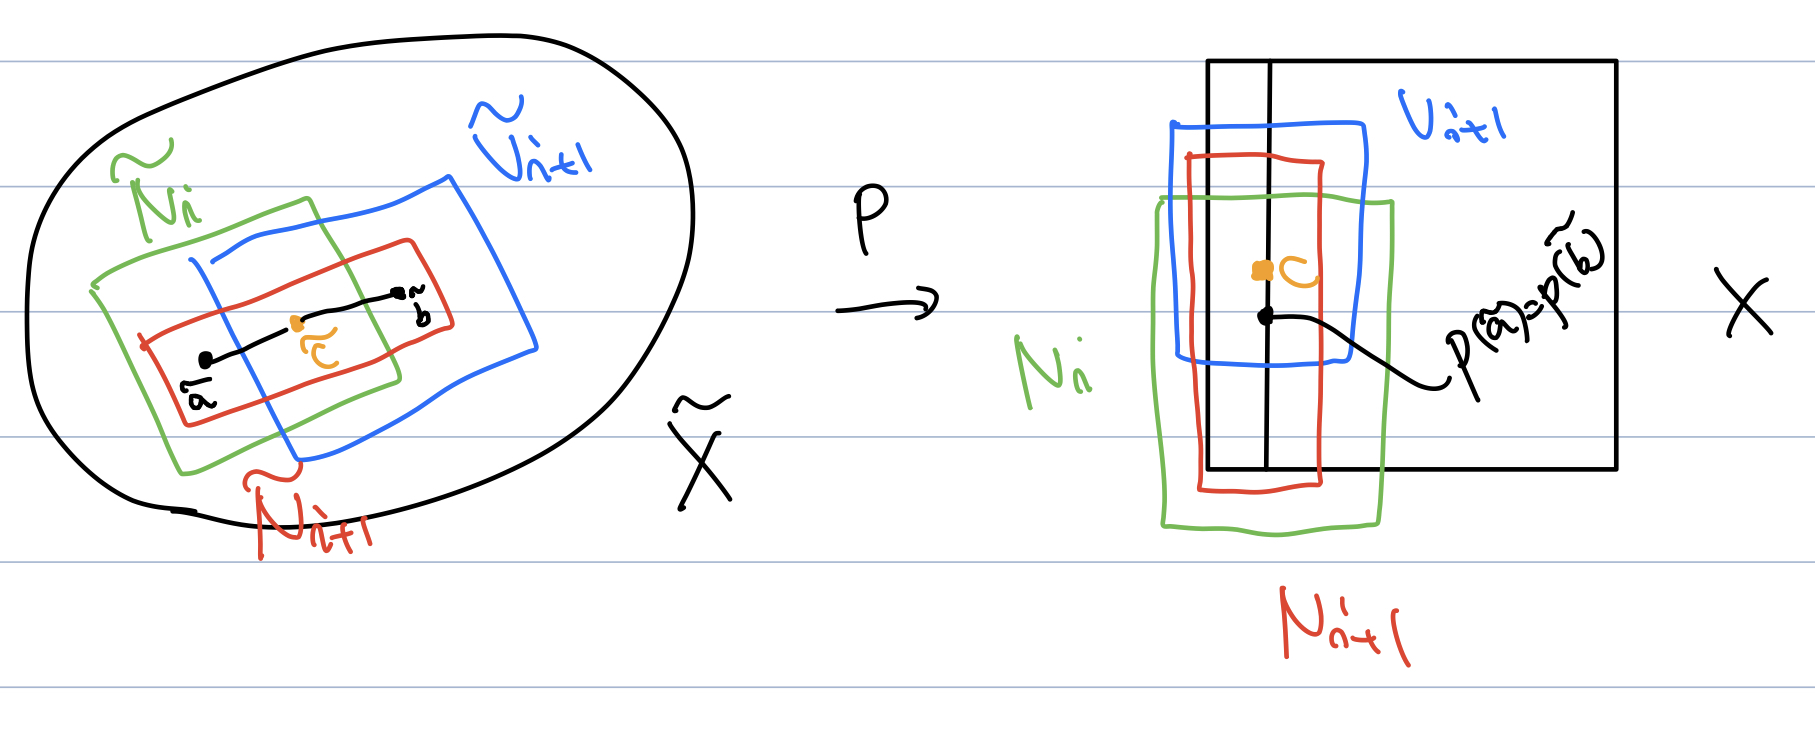
\includegraphics[width=.5\linewidth]{problem5_injective.jpeg}
        \caption{Problem 5(Injectivity)}
        \label{fig:problem5_injective}
      \end{figure}
      $c$ and $p(\tilde{a})$ are path connected in $N_i$, and $c$ and $p(\tilde{b})$ are path connected in $V_{i + 1}$.
      Thus $\tilde{c}$ and $\tilde{a}$ are path connected in $\tilde{N}_i$ and $\tilde{c}$ and $\tilde{b}$ are path connected in $\tilde{V}_{i + 1}$.
      Consider the path $\gamma$ from $\tilde{a}$ to $\tilde{b}$ formed by the two paths to $\tilde{c}$.
      A small neighborhood of $\tilde{c}$ is mapped homeomorphically to a neighborhood of $c$.
      However, this implies that one of $p(\tilde{a})$ or $p(\tilde{b})$ will be located above $c$ and the other one will be located below $c$.
      This is a contradiction because $p(\tilde{a}) = p(\tilde{b})$.
    \item
      Surjective?
      Let $x \in N_{i + 1}$.
      \begin{itemize}
        \item
          Case 1: $x \in V_{i + 1}$.
          Then there exists an $\tilde{x} \in \tilde{V}_{i + 1}$ such that $p(\tilde{x}) = x$.
          Moreover, $\tilde{x} \in p^{-1}(N_{i + 1})$.
          Therefore, $\tilde{x} \in \tilde{N}_{i + 1} = p^{-1}(N_{i + 1}) \cap (\tilde{N}_i \cup \tilde{V}_{i + 1})$.
        \item
          Case 2: $x \in N_i$.
          Then there exists an $\tilde{x} \in \tilde{N}_i$ such that $p(\tilde{x}) = x$.
          Moreover, $\tilde{x} \in p^{-1}(N_{i + 1})$.
          Therefore, $\tilde{x} \in \tilde{N}_{i + 1} = p^{-1}(N_{i + 1}) \cap (\tilde{N}_i \cup \tilde{V}_{i + 1})$.
      \end{itemize}
    \item
      Continuous?
      $p$ is defined to be continuous, so the restriction of it must be continuous.
    \item
      Continuous inverse?
      Since $p\mid_{\tilde{N}_{i + 1}}$ is bijective, the inverse exists.
      Since the inverses of $p$ restricted to $N_i$ and $V_{i + 1}$ are both continuous, the inverse of $p\mid_{\tilde{N}_{i + 1}}$ is continuous by the pasting lemma.
  \end{itemize}

  We will obtain $N_k, \tilde{N}_k$ after $k$ steps, and $N_k$ is a neighborhood of the left edge such that $p$ maps $\tilde{N}_k$ into $N_k$ homeomorphically.
\end{proof}

\begin{exer}{(Problem 7, Chapter 1.3)}
  Let $Y$ be the quasi-circle in the figure in the textbook.
  Collapsing the segment of $Y$ in the $y$-axis to a point gives a quotient map $f: Y \rightarrow S^1$.
  Show that $f$ does not lift to the covering space $\mathbb{R} \rightarrow S^1$, even though $\pi_1(Y) = 0$.
  Thus local path-connectedness of $Y$ is a necessary hypothesis in the lifting criterion.
\end{exer}

\begin{proof}
  We will use the lifting criterion (Proposition 1.33) and its proof in the textbook.
  The only missing property among the required ones is that $Y$ is not locally path connected.
  By the first part of the proof (up to ``This shows that $\tilde{f}$ is well-defined"), we know that if there exists $\tilde{f}$, it must be the function that the first part of the proof describes.
  Note that the first part does not require that $Y$ be locally path connected.
  We will prove that the defined mapping is not continuous.

  Let $x_0 = 1 \in S^1$.
  Let $y_0 \in Y$ be the point that gets mapped to $x_0$.
  Let $y$ be the point on the intersection of the $[-1, 1]$ segment and the circle, and let $\gamma$ denote the path from $y_0$ to $y$.
  Then $\widetilde{f \circ \gamma}(y)$ is somewhere around $-0.6$ in $\tilde{X}$.
  (See Figure \ref{fig:problem7}.)
  \begin{figure}
    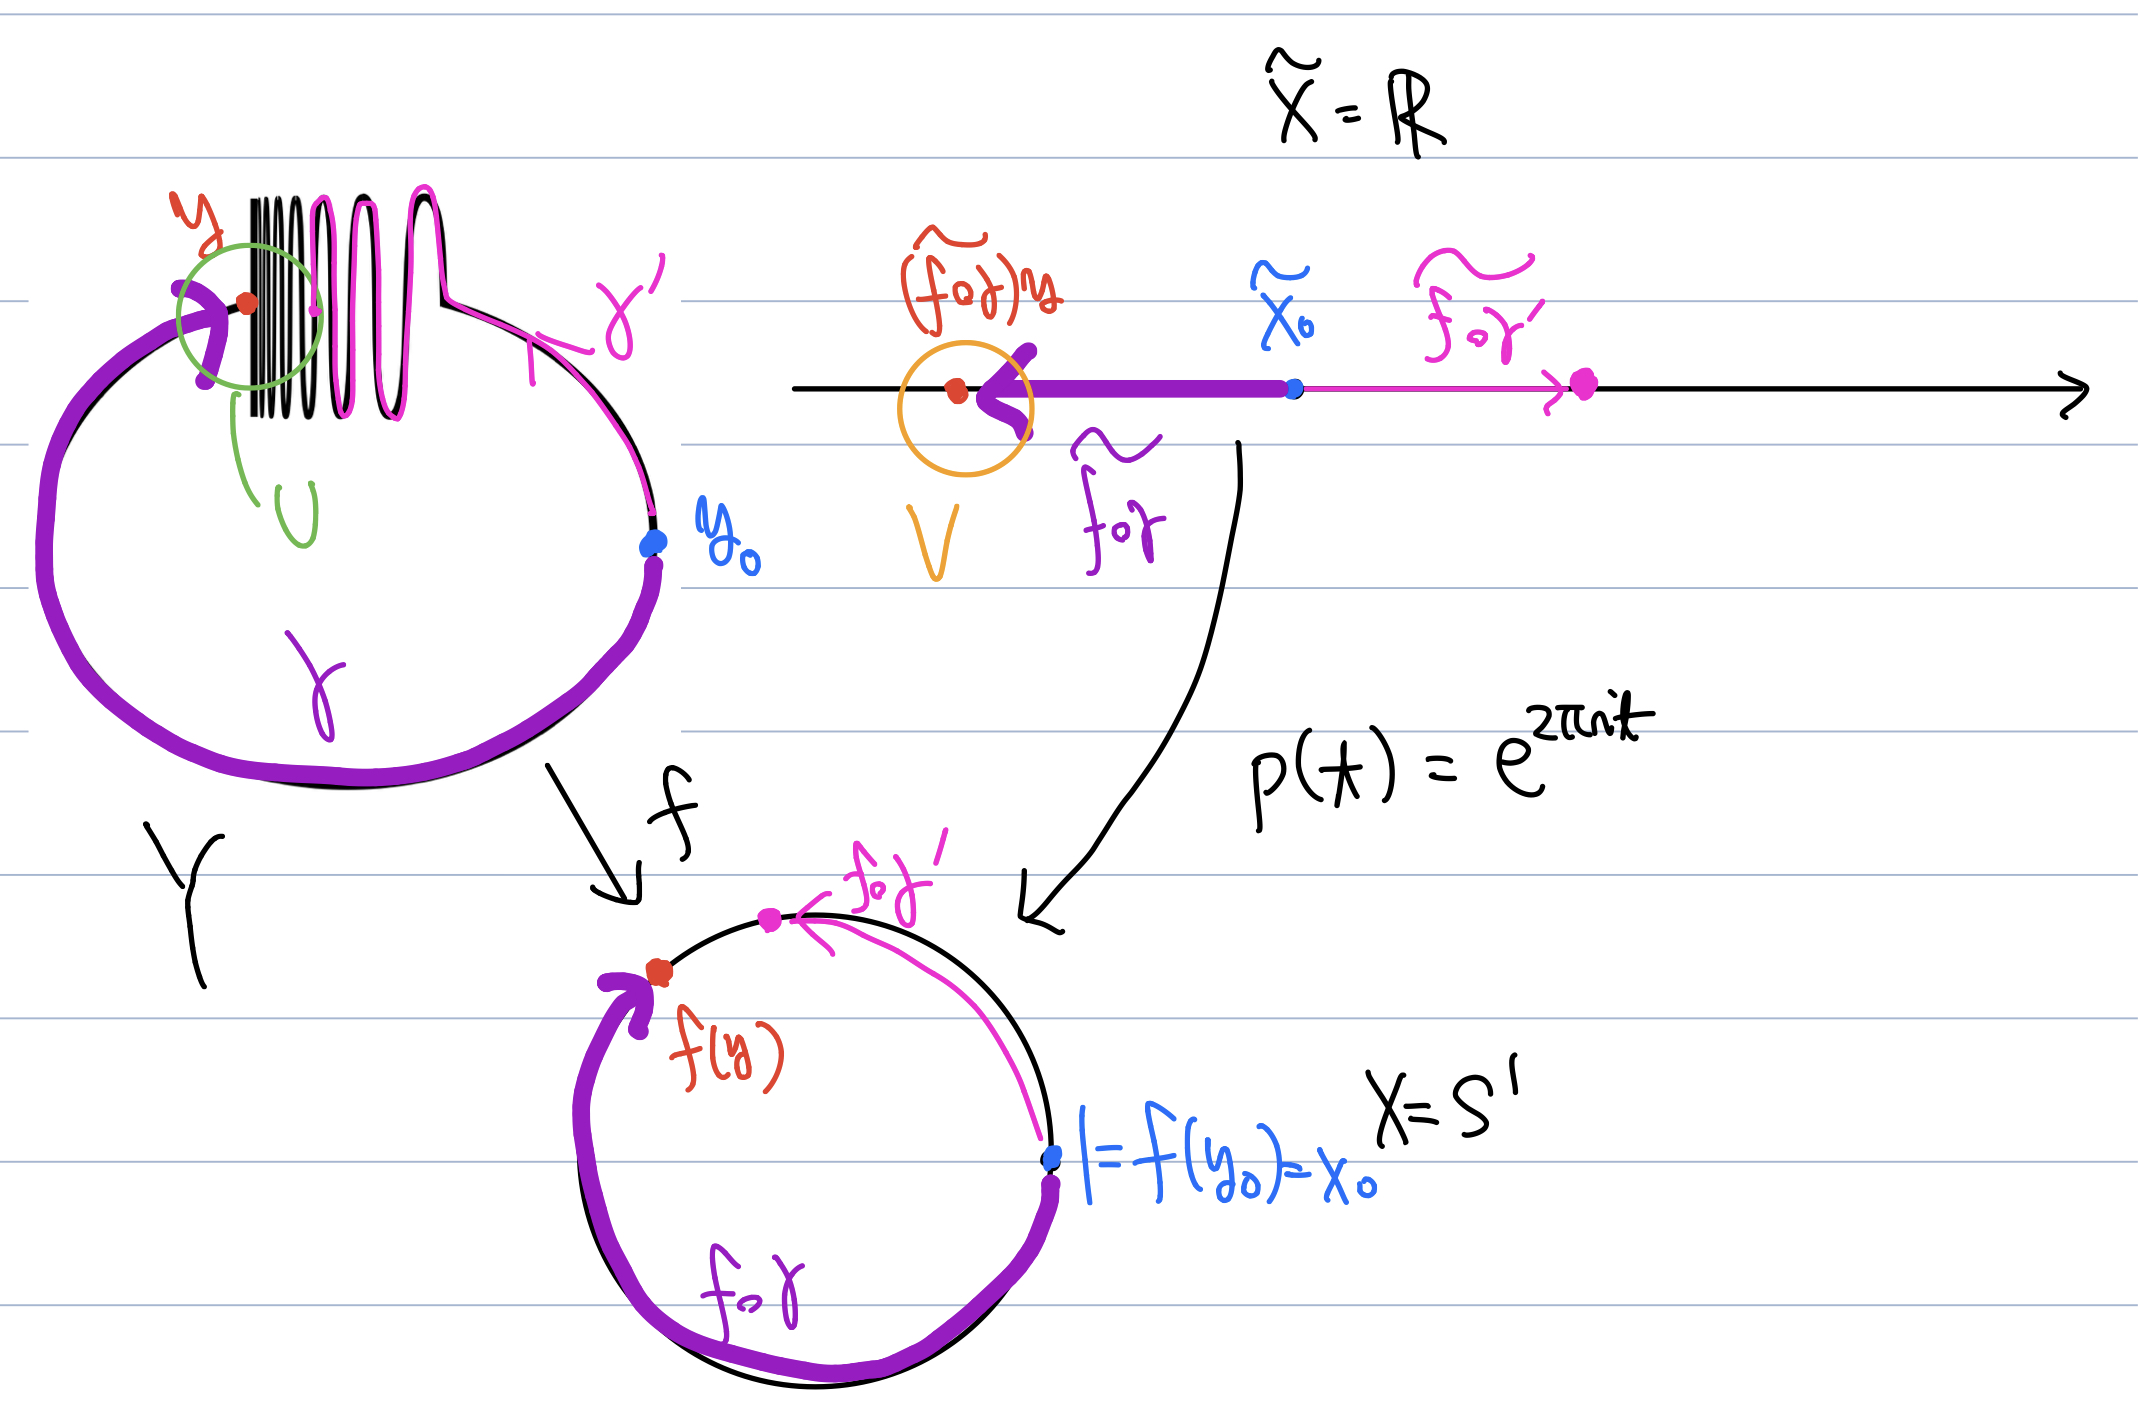
\includegraphics[width=.5\linewidth]{problem7.jpeg}
    \caption{Problem 7}
    \label{fig:problem7}
  \end{figure}
  Let $V = (\widetilde{f \circ \gamma}(y) - 0.01, \widetilde{f \circ \gamma}(y) + 0.01)$.
  (A small neighborhood around $\widetilde{f \circ \gamma}(y)$ that does not include $0$.)

  A necessary condition for $\tilde{f}$ to be continuous is that there exists a neighborhood $U \subset Y$ of $y$ such that $\tilde{f}(U) \subset V$.
  (For instance, Theorem 18.1 on P.104 from Topology by Munkres.)

  Let $U \subset Y$ be a neighborhood of $y$.
  Then it certainly contains some point of $y = \sin (1/x)$.
  Let $\gamma'$ denote the path from $y_0$ to such a point in $Y$.
  Then $\tilde{f}$ maps the point to somewhere around $0.3$ in $\tilde{X}$.
  In other words, $\widetilde{f \circ \gamma}(1) \notin V$, so $\tilde{f}(U) \not\subset V$.

  Therefore, $\tilde{f}$ is not continuous.
  By the uniqueness discussed in the first part of the proof for Proposition 1.33, we conclude that there does not exist a lift of $f$.
\end{proof}

\begin{exer}{(Problem 11, Chapter 0)}
  Show that $f: X \rightarrow Y$ is a homotopy equivalence if there exist maps $g, h: Y \rightarrow X$ such that $fg \simeq \Id$ and $hf \simeq \Id$.
  More generally, show that $f$ is a homotopy equivalence if $fg$ and $hf$ are homotopy equivalences.
\end{exer}

\begin{proof}
  We will only show the first part because we will only use the first part for Problem 8.

  Let $F$ be a homotopy between $f \circ g$ and $\Id$, and let $H$ be a homotopy between $h \circ f$ and $\Id$.
  Let $G: X \times I \rightarrow X$ be defined such that 

  \begin{align*}
    G_t &= \begin{cases}
      H_{1 - 3t} \circ g \circ f & (t \in [0, 1/3]) \\
      h \circ F_{3t - 1} \circ f & (t \in [1/3, 2/3]) \\
      H_{3t - 2} & (t \in [2/3, 1]).
    \end{cases}
  \end{align*}

  \begin{itemize}
    \item
      $G$ is well-defined and continuous.
      \begin{itemize}
        \item
          $G_{1/3} = H_0 \circ g \circ f = h \circ f \circ g \circ f$.
        \item
          $G_{1/3} = h \circ F_0 \circ f = h \circ f \circ g \circ f$.
        \item
          $G_{2/3} = h \circ F_1 \circ f = h \circ f$.
        \item
          $G_{2/3} = H_0 = h \circ f$.
      \end{itemize}
      By the pasting lemma, $G$ is continuous.
    \item
      When $t = 0$, $G(x, 0) = H_1 \circ g \circ f = g \circ f$.
    \item
      When $t = 1$, $G(x, 1) = H_1 = \Id$.
  \end{itemize}

  Therefore, $G$ is a homotopy between $g \circ f$ and $\Id_X$.
  Thus $f \circ g$ is homotopic to $\Id_Y$ and $g \circ f$ is homotopic to $\Id_X$.
  Hence, $f$ and $g$ are homotopy equivalences.
\end{proof}

\begin{exer}{(Problem 8, Chapter 1.3)}
  Let $\tilde{X}$ and $\tilde{Y}$ be simply-connected covering spaces of the path-connected, locally path-connected spaces $X$ and $Y$.
  Show that if $X \simeq Y$ then $\tilde{X} \simeq \tilde{Y}$.
\end{exer}

\begin{proof}
  \begin{figure}
    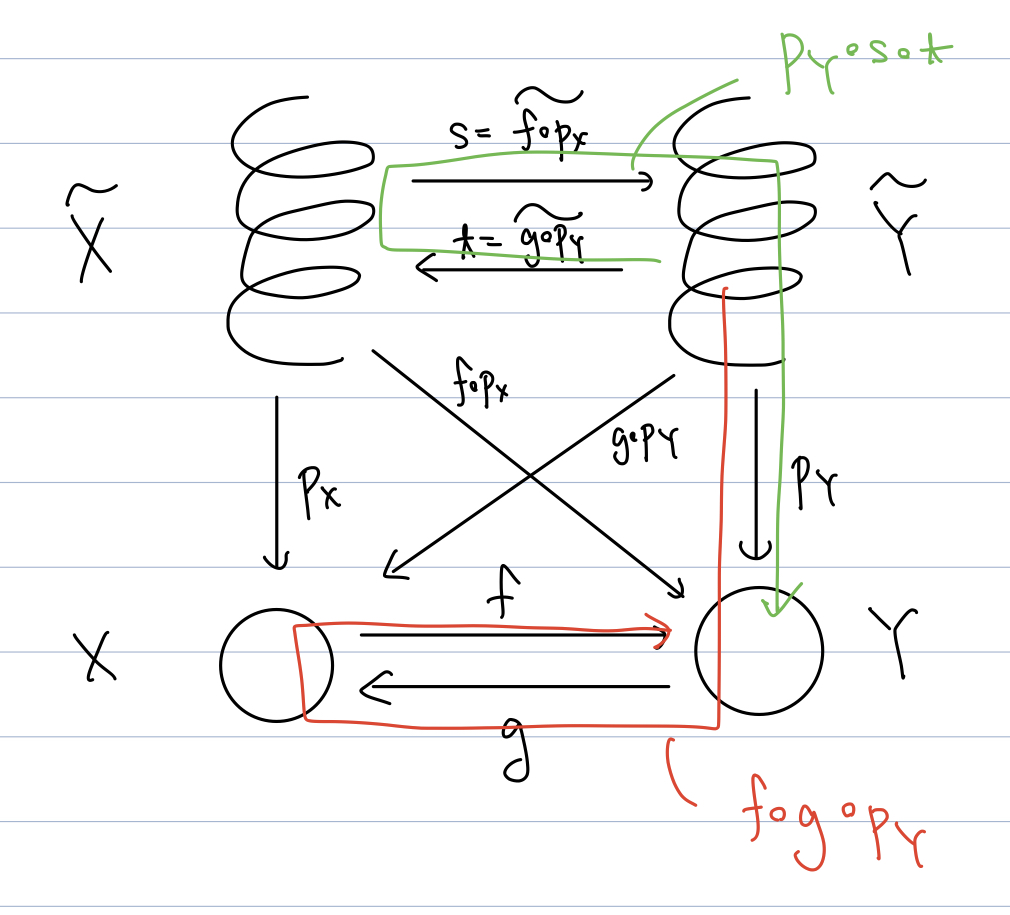
\includegraphics[width=.5\linewidth]{problem8_diagram.jpeg}
    \caption{Problem 8}
    \label{fig:problem8_diagram}
  \end{figure}
  Let $f, g$ be homotopy equivalences as defined in Figure \ref{fig:problem8_diagram}.
  By Proposition 1.33, we can lift $f \circ p_X$ and $g \circ p_Y$ as defined in Figure \ref{fig:problem8_diagram}.
  This works because $\pi_1(\tilde{X}) = \pi_1(\tilde{Y}) = 0$.
  Let $s = \widetilde{f \circ p_X}, t = \widetilde{g \circ p_Y}$.

  Since $f \circ g$ is homotopic to $\Id_Y$, $f \circ g \circ p_Y$ is homotopic to $\Id_Y \circ p_Y = p_Y$.
  Let $F: \tilde{Y} \times I \rightarrow Y$ be a homotopy between them such that $F_0 = f \circ g \circ p_Y$ and $F_1 = p_Y$ where $F_t$ denotes the function $\tilde{y} \mapsto F(\tilde{y}, t)$.
  We will apply Proposition 1.30 (the homotopy lifting property) to lift $F$ such that $\tilde{F}_0 = s \circ t$.
  This is possible because we have:
  \begin{itemize}
    \item
      A covering space $p_Y: \tilde{Y} \rightarrow Y$.
    \item
      A homotopy $F_t: \tilde{Y} \times I \rightarrow Y$.
    \item
      We have $f \circ g \circ p_Y = p_Y \circ s \circ t$.
      (See Figure \ref{fig:problem8_diagram}.)
      Therefore, $s \circ t: \tilde{Y} \rightarrow \tilde{Y}$ lifts $F_0$.
  \end{itemize}

  If $\tilde{F}_1$ is the identity map on $\tilde{Y}$, then that will imply that $s \circ t$ is homotopic to the identity map.
  However, this may not be true.

  Let $r: \tilde{Y} \rightarrow \tilde{Y}$ such that $r(\tilde{y}) = \tilde{F}(\tilde{y}, 1)$ for any $\tilde{y} \in \tilde{Y}$.
  Let $y_0 \in Y$ be given arbitrarily.
  Choose $\tilde{y_0} \in Y$ such that $p_Y(\tilde{y_0}) = y_0$.
  Then $\tilde{y_0}, r(\tilde{y_0})$ are both points in $\tilde{Y}$.
  Let $k: \tilde{Y} \rightarrow \tilde{Y}$ be a lift of $p_Y$ such that $k(r(\tilde{y_0})) = \tilde{y_0}$.  This is possible by Proposition 1.33 because we have:
  \begin{itemize}
    \item
      A covering space $p_Y: (\tilde{Y}, \tilde{y_0}) \rightarrow (Y, y_0)$.
    \item
      A map $p_Y: (\tilde{Y}, r(\tilde{y_0})) \rightarrow (Y, y_0)$.
      This makes sense because
      \begin{align*}
        p_Y(r(\tilde{y_0}))
          &= p_Y(\tilde{F}(\tilde{y_0}, 1)) \\
          &= F(\tilde{y_0}, 1) \\
          &= p_Y(\tilde{y_0}) \\
          &= y_0.
      \end{align*}
    \item
      $\tilde{Y}$ is simply connected, so both $\pi_1(\tilde{Y}, \tilde{y_0})$ and $\pi_1(\tilde{Y}, r(\tilde{y_0}))$ are trivial.
    \item
      $Y$ is path connected and locally path connected.
  \end{itemize}

  We claim that $k \circ r = \Id_{\tilde{Y}}$.
  \begin{itemize}
    \item
      Claim 1: $k \circ r$ is a lift of $p_Y$.
      $p_Y \circ k = p_Y$ because $k$ is a lift of $p_Y$, and $p_Y \circ r = p_Y$ because $r$ is a lift of $p_Y$.
      Thus $p_Y \circ (k \circ r) = (p_Y \circ k) \circ r = p_Y \circ r = p_Y$, so $k \circ r$ is a lift of $p_Y$.
    \item
      Claim 2: $k \circ r = \Id_{\tilde{Y}}$.
      $k \circ r$ is a lift of $p_Y$ that maps $\tilde{y_0}$ to $(k \circ r)(\tilde{y_0}) = \tilde{y_0}$.
      On the other hand, $\Id_{\tilde{Y}}$ is clearly a lift of $p_Y$ that maps $\tilde{y_0}$ to $\tilde{y_0}$.
      By Proposition 1.34(the unique lifting property), the two lifts must be identical.
      Therefore, $k \circ r = \Id_{\tilde{Y}}$.
  \end{itemize}

  By the homotopy $\tilde{F}$, $s \circ t$ is homotopic to $r$.
  Therefore, $k \circ (s \circ t)$ is homotopic to $k \circ r$.
  Since $k \circ r = \Id_{\tilde{Y}}$, $(k \circ s) \circ t$ is homotopic to $\Id_{\tilde{Y}}$.

  Similarly, there must exist an $r': \tilde{X} \rightarrow \tilde{X}$ such that $t \circ s$ is homotopic to $r'$.
  Moreover, there must exist a $k': \tilde{X} \rightarrow \tilde{X}$ such that $r' \circ k = \Id_{\tilde{X}}$ using the same argument.

  Therefore, $t \circ (s \circ k) = (t \circ s) \circ k$ is homotopic to $r' \circ k = \Id{\times{X}}$.

  By the first part of Problem 11 in Chapter 0, $t: \tilde{Y} \rightarrow \tilde{X}$ is a homotopy equivalence.
\end{proof}


\end{document}


